\subsubsection{الگوی \lr{Watchdog}}
\label{archSafeWatchDogSec}
\begin{RTL}
این الگو \cite{ref4}
یک روش سبک و کم‌هزینه برای اطمینان از عملکرد صحیح فرآیندهای
محاسبات داخلی است. برخلاف \nameref{archSafeSanityChkSec}
که خروجی سیستم را با استفاده از حسگرهای خارجی نظارت می‌کند،
الگوی \lr{Watchdog} بررسی می‌کند که محاسبات
به درستی و به موقع انجام شوند. این الگو پوشش خطای حداقلی ارائه می‌دهد
و عمدتاً خطاهای پایه زمانی و گیر افتادن احتمالی را شناسایی می‌کند.
این الگو اغلب با الگوهای ایمنی دیگر ترکیب می‌شود تا قابلیت اطمینان سیستم
را افزایش دهد، به‌ویژه در برنامه‌های حساس به زمان که محاسبات
باید ضرب‌الاجل‌های دقیقی را رعایت کنند.
\end{RTL}
\begin{figure}[h!]
\centering
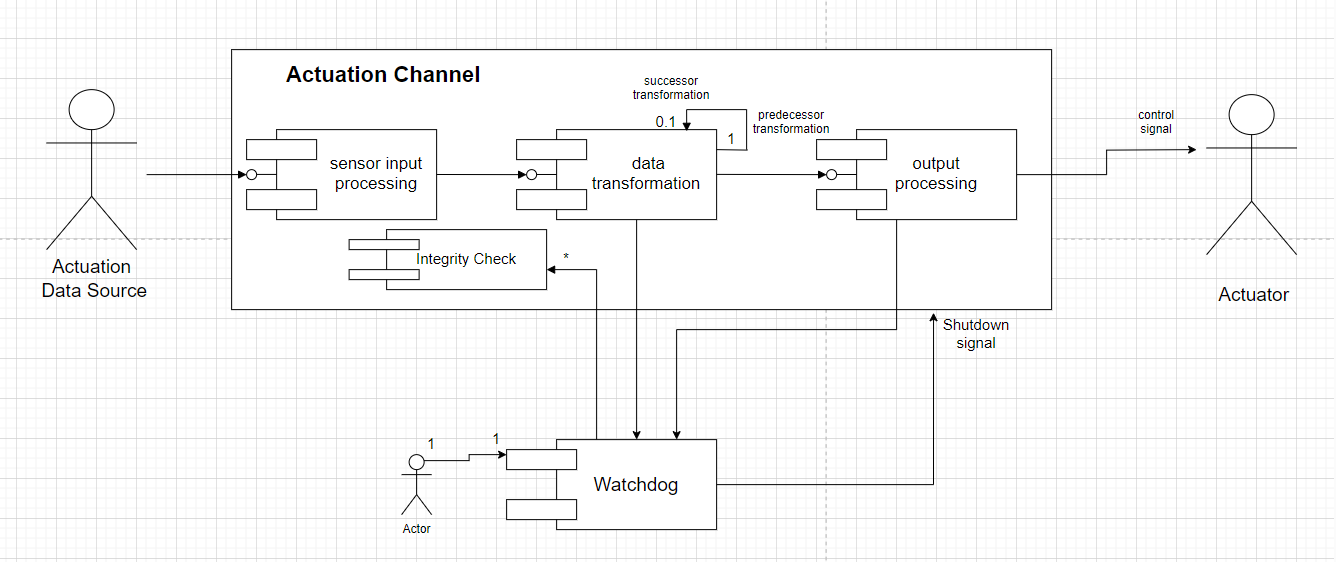
\includegraphics[scale=0.5]{images/third/watchdog.png}
\caption{ساختار الگوی \lr{Watchdog}}
\end{figure}